\chapter{Feasibility-aware plan adaptation in humanoid gait generation}
\label{ch:FAPA}
In Chapters \ref{ch:ISMPC} and \ref{ch:humanoid-motion-generation-WoS} we have
seen how to design a scheme for humanoid locomotion, which allow 
the robot to perform walking motions in complex scenarios. One of the
characteristics that marks the presented framework is the separation into a 
footstep planning phase (based on RRT*), and a Model Predictive Control (MPC)
gait generation algorithm. Most available schemes used for humanoid walking 
rely on such separation, lightening the computational load on the control side,
and allowing it to run in real-time. Nevertheless, with this kind of design,
the planner is unaware of the underlying dynamics, and the controller is unaware
of any disturbances acting on the robot.

In this chapter, we present an on-line
Feasibility-Aware Plan Adaptation (FAPA) module which can locally adapt
footsteps (positions, timings and orientation) in such a way that to guarantee
feasibility of the subsequent Intrinsically Stable MPC (IS-MPC) stage.
Indeed, because our architecture is based on IS-MPC (Chapter \ref{ch:ISMPC}),
which involves an explicit stability constraint ensuring the boundedness of 
the CoM trajectory with respect to the ZMP, it is possible to use its
feasibility region (i.e., the state space region for which the constrained
QP admits a solution) to enhance the capabilities of the scheme itself.
Two examples of such strategy rely on adapting the time of the first step 
\cite{Smaldone2021FeasibilityDrivenSTA} and allowing for non-convex regions 
\cite{Habib2022HandlingNonConvex}. 

With the FAPA module, which depends on the system state and the dynamics
of the chosen template dynamic model, we obtain the generality given by
nonlinear constraints without sacrificing
much performance as the number of variables in FAPA is much lower than
that of the variables of the MPC, making it very fast and capable of working
in real time. Furthermore, we explore the inclusion of integer variables,
further increasing the range of situations that can be covered. Note that while modules for online
footstep adaptation using nonlinear
optimization have been proposed \cite{Ding2019IROS}, they do not work in
conjunction with MPC. Our approach is not only designed to work along
with the MPC module, but it specifically aimed at enhancing its capabilities.

We present two versions of the proposed FAPA scheme: one with a fixed regions
assignment for placing the footstep and another one where the regions are
selected automatically through mixed-integer programming.

\begin{figure}
    \centering
    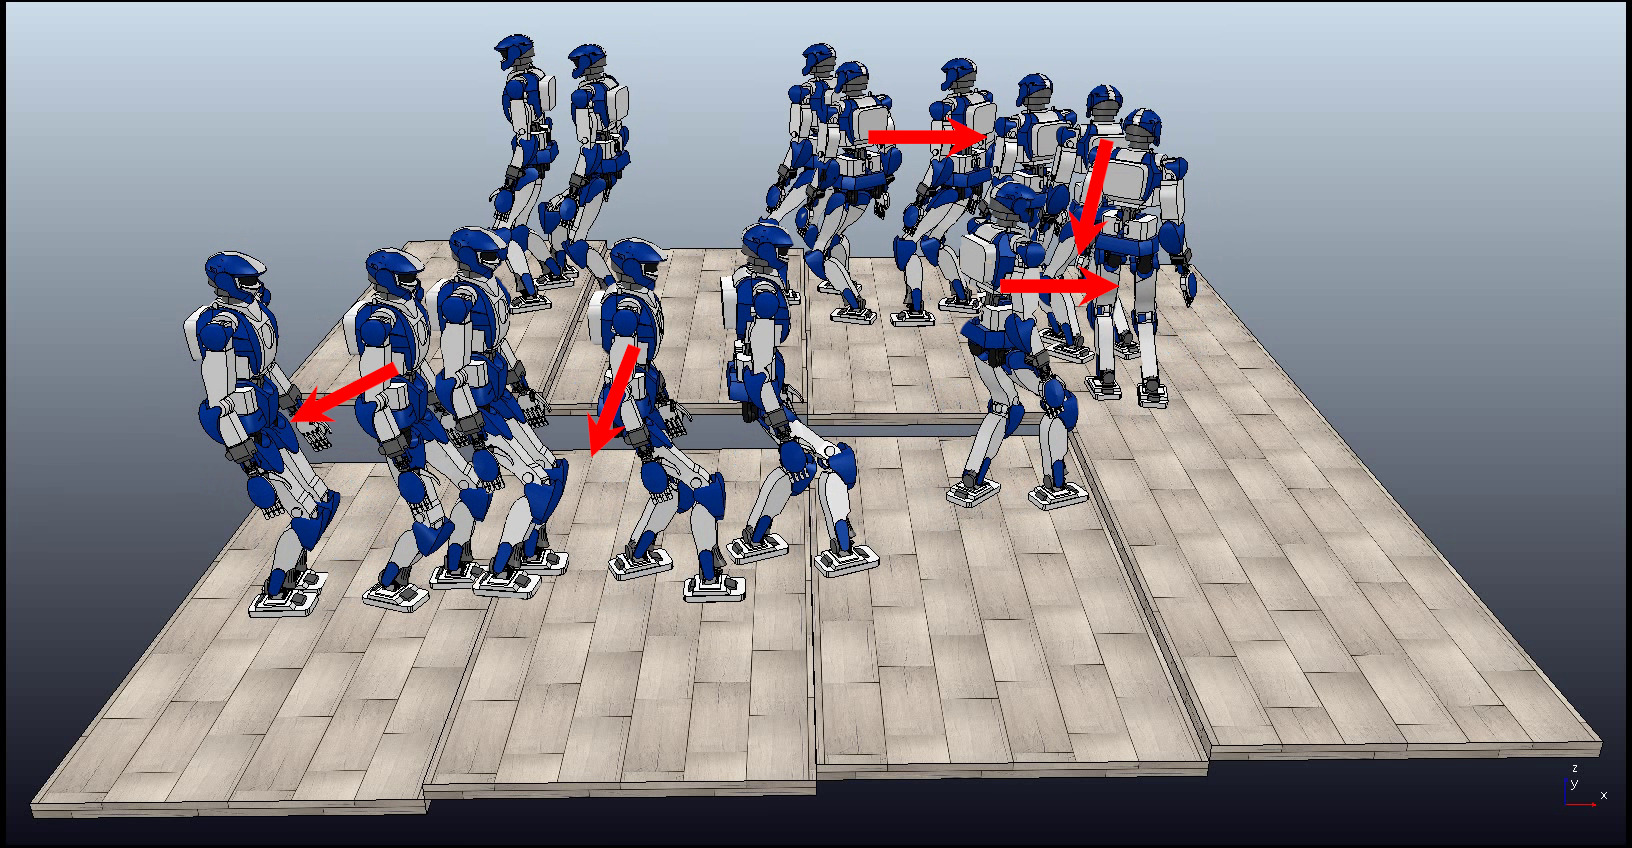
\includegraphics[trim={0.5cm 1.5cm 2cm 0.1cm},clip,width=0.9\columnwidth]{figures/strobo-staircase-with-pushes-2.jpeg}
    \caption{An example simulation using the proposed architecture: the robot is walking along a staircase while being subject to multiple pushes. The adaptation module modifies position, orientation and timing of the footsteps real-time to guarantee a successful execution.}
    \label{fig:FAPA:two-patches-mixed-integer-snapshots}
\end{figure}

\section{Problem formulation} 
\label{sec:FAPA:ProblemFormulation}
The proposed architecture is shown in Fig.~\ref{fig:FAPA:block_scheme}.
An external candidate plan is provided, which in this chapter will be either
a basic plan to demonstrate simple motions, or a plan generated by randomized
exploration (Chapter \ref{ch:humanoid-motion-generation-WoS})
for more complex environments.
A subplan, i.e., a portion of the candidate plan, is given as input to the
scheme at each timestep.

\begin{figure}
    \centering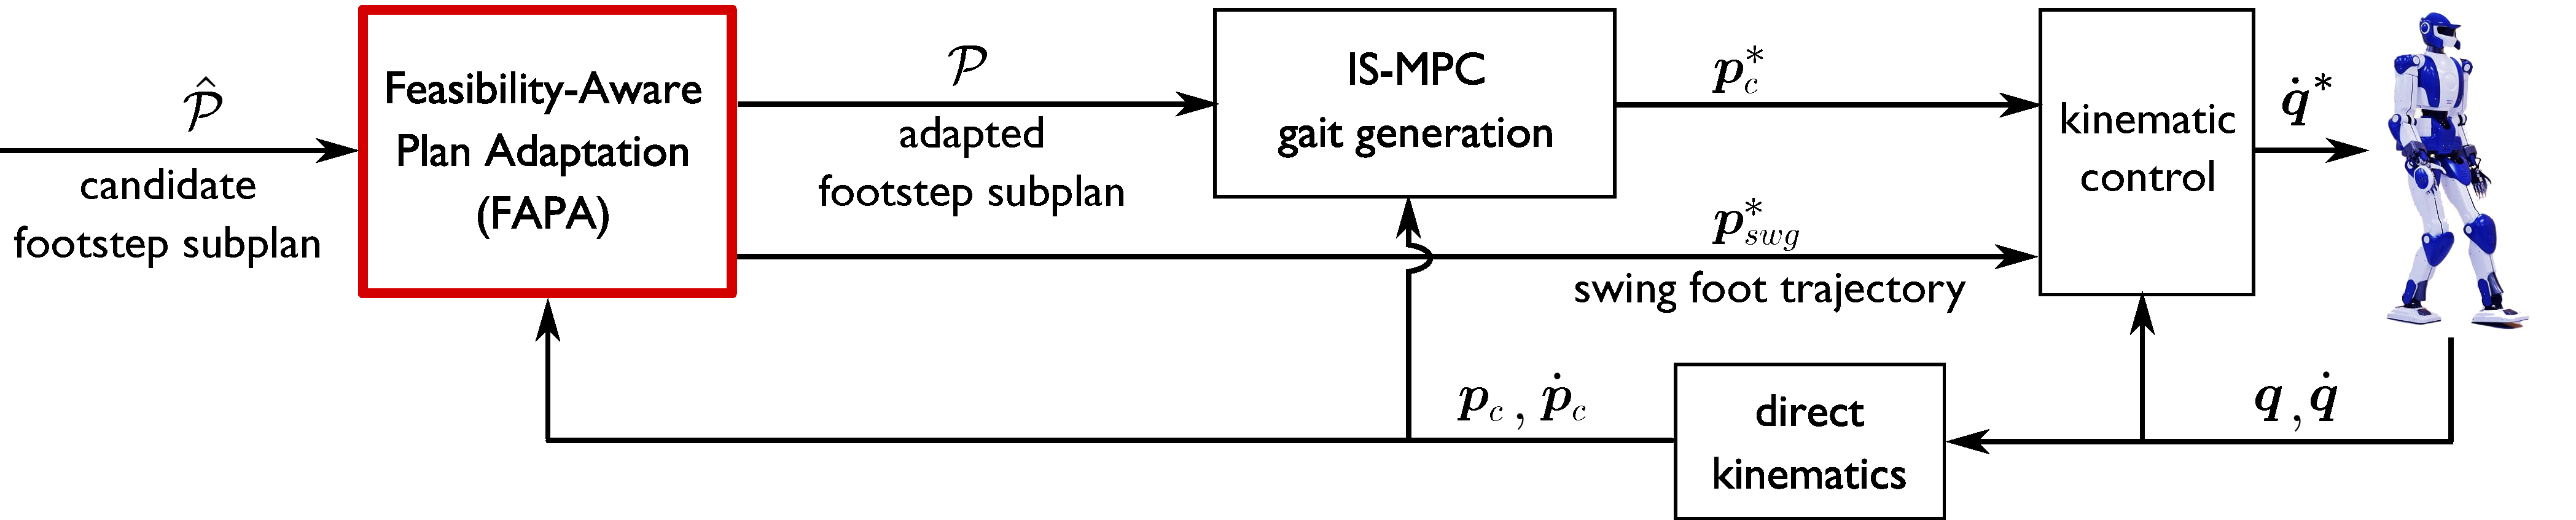
\includegraphics[width=\textwidth]{figures/BlockScheme-NLP-STA.pdf}
    \caption{A block scheme of the proposed architecture. The candidate footstep subplan $\mathcal{\hat{P}}$ is adapted by the FAPA module, guaranteeing the feasibility of IS-MPC. The IS-MPC module receives the adapted footstep subplan $\mathcal{P}$, and generates a desired trajectory of the CoM $\bm{p^*}_c$, which is used by the kinematic controller, together with the desired trajectory of the swing foot $\bm{p^*}_{\rm swg}$, to generate the desired joint velocities $\dot{\bm{q^*}}$.}
    \label{fig:FAPA:block_scheme}
    \end{figure}

The basic components of the considered scheme are:
\begin{itemize}
    \item a Feasibility-Aware Plan Adaptation (FAPA) block, that can modify locally
        the high-level footstep plan;
    \item an IS-MPC gait generation block (Chapter \ref{ch:ISMPC}) that generates CoM/ZMP trajectories based
        on the output of FAPA;
    \item a kinematic controller that realizes at the joint level the generated
        CoM and swing foot trajectories.
\end{itemize}

While the high-level footstep plan is designed considering the humanoid's
kinematic limitations, it is entirely unaware of its dynamics and is not
informed by the robot state since it is fully generated off-line.
To make up for this deficiency, the FAPA module performs a local adaptation of
the planned footsteps before these enter the IS-MPC stage. 

This adaptation is based on a {\em gait feasibility constraint} that guarantees
feasibility of the next IS-MPC stage while trying to match the original plan.
It can concurrently change the footstep positions, orientations, as well as
step timings. 

To formulate this constraint, we leverage the feasibility region of IS-MPC
(i.e., the subset of the state space where the problem is feasible at a given
time), and define it in an implicit form with the nonlinear dependency on the footstep
positions, orientations, and step timings.

The fact that the feasibility of the MPC can be efficiently captured by
the expression of this constraint is a crucial aspect of the formulation,
because it means that the scheme can harness the power of nonlinear
optimization without burdening the MPC itself, which remains linear and can
run at a high rate. The nonlinear optimization part is external to the MPC,
which allows the number of variables to be kept small and thus to keep the
computation time manageable.

We propose two versions of the FAPA module, that differ by the optimization
problem required for their implementation. In particular, the first version
only uses continuous optimization, while the second one also employs discrete
variables and is formulated as a Mixed Integer Nonlinear Program (MINLP).
Being the latter very general it can be used to account for more adaptation
scenarios, e.g., in which the footsteps can also be moved to different terrain
patches than the ones assigned by the high-level planner. As will be discussed
extensively in Sect.~\ref{sec:FAPA:Simulations}, the second version is more
demanding in terms of computation time, but we present it as a proof of
concept as we strongly believe it can be made to work in real time with proper
code optimization.

\section{Preliminaries}
\label{sec:FAPA:Preliminaries}
In this section we describe the environment and the structure of the footstep
plan used in our scheme.

\subsection{Environment}
The considered environment is a world of stairs, i.e., constituted by flat
horizontal regions. The robot is allowed to walk across different regions if
these are relatively close in height, and if there is sufficient available
surface to step on them, otherwise they will constitute obstacles to be avoided.

The arrangement of these regions is assumed to be known, and it is processed
and encoded in the following way:
\begin{itemize}
    \item regions are reduced in size so that they represent the collision-free
        area available for the center of the footprint. This is done by
        performing a Minkowski difference between each flat region and the
        area swept by a footprint (accounting for all possible footstep orientations);
    \item after reduction, non-convex regions are subdivided into
        non-overlapping convex polytopic {\em patches}.
\end{itemize}
A patch $P$ is identified by the inequality
\begin{equation*}
\bfA(P) \bfp \le \bfb(P),
\end{equation*}
where $\bm{A}(P) \in \mathbb{R}^{V(P) \times 2}$ and
$\bm{b}(P) \in \mathbb{R}^{V(P)} $ define a polytope (with $V(P)$ vertices)
and $\bfp = (x, y)^\top$ is a generic 2D point. 
In this way, non-polytopic portions of ground (e.g., round edges) are
approximated, but the number of vertices can be arbitrarily large.
Since each patch $P$ is flat, its height is denoted simply as $z(P)$.

\subsection{Footstep plan}
The high-level footstep plan is a sequence of {\em candidate footsteps}
$\hat\bff$, each identified by the tuple
$\hat\bff = (\hat x_f, \hat y_f, \hat z_f, \hat\theta_f, \hat T_{\rm ss}, \hat T_{\rm ds})$.
For each planned footstep $\hat\bff$

\begin{itemize}
    \item $\hat x_f$, $\hat y_f$ and $\hat z_f$ are the coordinates of its center;
    \item $\hat\theta_f$ is its orientation around the $z$ axis;
    \item $\hat T_{\rm ds}$ and $\hat T_{\rm ss}$ are the durations of its  double support and single support phases, respectively;
    \item we denote by $\Pi(\hat\bff)$ the patch that contains the footstep, i.e., the patch $P$ such that\footnote{Note that this patch is unique because the environment is subdivided into non-overlapping patches.}
    \[
    \left[\hat{x}_f, \hat{y}_f\right]^\top \in P,\quad \hat{z}_f = z(P).
    \]
\end{itemize}

The footstep plan $\mathcal{\hat P}$ is computed off-line, and at each time
$t_k$ a subplan $\mathcal{\hat P}^l$ of size $F+1$ is extracted, where $l$ is
the index of the first footstep of the current subplan (at $t_k$), and $F$ a
fixed parameter. The subplan contains the next $F$ candidate footsteps:
\begin{equation*}
\mathcal{\hat P}^l = \left\{
\hat\bff^{l},\,\dots,\,\hat\bff^{l+F}
\right\}.
\end{equation*}
The FAPA block, which performs footsteps adaptation, modifies
$\mathcal{\hat P}^l$ in the adapted subplan $\mathcal{P}^l$, i.e., in the input
of the IS-MPC block
\begin{equation*}
    \mathcal{P}^l = \left\{
    \bff^{l},\,\dots,\,\bff^{l+F}
    \right\}.
\end{equation*}

After every iteration, if adaptation took place (i.e., $\mathcal{P}^l$ differs
from $\mathcal{\hat P}^l$), the algorithm performs a {\em footstep plan
override}, i.e., the corresponding portion of the high-level footstep plan
is substituted with the adapted subplan $\mathcal{P}^l$. Note that the
remaining part of the plan (after the index $l+F$) is unchanged, so if the
adaptation makes the robot stray from the initial path it will later try to
catch up. This behavior is often acceptable, but might sometimes be undesirable,
and can be improved in future versions if we allow the high-level planner
to replan on-line (see \cite{Cipriano2023RAS}).

\section{Feasibility-Aware Plan Adaptation}
\label{sec:FAPA:FeasibilityAwarePlanAdaptation}
In this following
section, we describe how to use the feasibility region to formulate a
constraint for the FAPA module, and thus ensure that the output of FAPA can be
used by IS-MPC to construct a feasible QP.
The FAPA module runs in real-time and performs a local adaptation of the
subplan $\mathcal{\hat P}^l$, including their timing. We now describe the
constraints and the optimization problems that define the adaptation procedure.

\subsection{Kinematic constraint}
The $j$-th footstep $\bff^{j}$ is ensured to be kinematically feasible by
limiting its displacement with respect to the previous footstep $\bff^{j-1}$.
In practice we constrain the geometric components of $\bff^{j}$ to be within
the \textit{admissible region}
\begin{equation}
\label{eq:FAPA:kinematic-constraint}
\begin{split}
\begin{bmatrix}
    \bm{n}_1^\top\left(\bm{p}_{xy}^{l+j} - \bm{p}_{xy}^{l+j-1} - \bm{R}(\theta_f^{l+j-1})\bm{v}_1\right) \\
    \vdots \\
    \bm{n}_V^\top\left(\bm{p}_{xy}^{l+j} - \bm{p}_{xy}^{l+j-1} - \bm{R}(\theta_f^{l+j-1})\bm{v}_V\right) \\
\end{bmatrix} \ge \bm{0},\\
    \Delta z^{\rm m} \le z_{l+j} - z_{l+j-1} \le \Delta z^{\rm M}, \\
    \Delta \theta^{\rm m} \le \theta_{l+j} - \theta_{l+j-1} \le \Delta \theta^{\rm M}, 
\end{split}
\end{equation}
with $\bm{R}\left(\theta_f^{l+j-1}\right)$ a 2D rotation matrix, $\bm{n}_i$ the vector
normal to the $i$-th segment of the convex region computed as
\begin{equation*}
    \bm{n}_i =
    \begin{bmatrix}
        0 & -1 \\ 1 & 0
    \end{bmatrix}
    \bm{R}\left(\theta_f^{l+j-1}\right)(\bm{v}_{i+1}-\bm{v}_i),
\end{equation*}
and $\bm{v}_i$ being the vertices defining the convex polygon (different
depending whether the support foot is left or right), shown in
Fig. \ref{fig:FAPA:kinematic-constraint}. Furthermore,
$\Delta_z^m$, $\Delta z^{\rm M}$, $\Delta \theta^{\rm m}$, and
$\Delta \theta^{\rm M}$ define limits for the foot reachability over vertical
displacement and relative orientation.

\begin{figure}
    \centering
    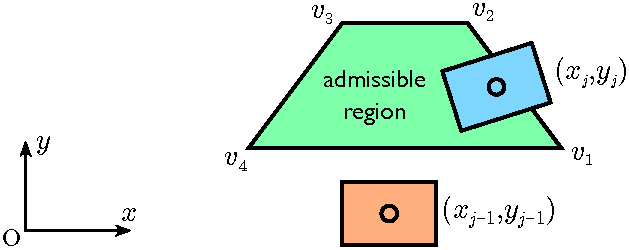
\includegraphics[width=0.7\textwidth]{figures/humanoids_kinconstr.pdf}
    \caption{Admissible region of the kinematic constraint in the $x$-$y$ plane.}
    \label{fig:FAPA:kinematic-constraint}
\end{figure}

\subsection{Timing constraint}
Single and double support duration are subject to minimum and maximum duration
constraints
\begin{equation}
    T_{\rm ss}^{\min} \le T_{\rm ss}^{l+j} \le T_{\rm ss}^{\max}, \quad T_{\rm ds}^{\min} \le T_{\rm ds}^{l+j} \le T_{\rm ds}^{\max},
    \label{eq:FAPA:timing-constraint}
\end{equation}
where the bounds $T_{\rm ds}^{\min}$, $T_{\rm ds}^{\max}$, $T_{\rm ss}^{\min}$, $T_{\rm ss}^{\max}$ are chosen in such a way to avoid excessively fast trajectories that might be difficult to track, as well as very slow steps that could result in quasi-static motion.

\subsection{Patch constraints}
\label{sec:FAPA:patch_constraint}
We describe alternative versions of this constraint, as we will later compare
the module using either of them, both in terms of the quality of the resulting
plan and of the computational load.
The first version of the constraint simply restricts the $(l+j)$-th footstep
to lie within its associated patch $\Pi(\bff^{l+j})$, which is the one
originally chosen by the high-level planner. This constraint can be written as
\begin{equation}
    \begin{cases}
		\bm{A}\left(\Pi\left(\bff^{l+j}\right)\right) \left[ x_f^{l+j} \ y_f^{l+j} \right]^\top \leq \bm{b}\left(\Pi\left(\bff^{l+j}\right)\right), \\
		z_f^{l+j} = z\left(\Pi\left(\bff^{l+j}\right)\right).
    \end{cases}
	\label{eq:FAPA:fixed_patch_constraint}
\end{equation}

The second version of the patch constraint allows the footstep to be moved
to a different patch. To entertain this possibility, we introduce binary
variables in order to formulate a mixed-integer constraint. This constraint
defines a logical implication in which, if a certain binary variable
$b_{l+j,\kappa}$ is {\em true}, then a linear constraint must be verified:
\begin{equation}
	b_{l+j,\kappa}=1 \Rightarrow 
	\begin{cases}
		\bm{A}\left(P^\kappa\right) \left[ x_f^{l+j} \ y_f^{l+j} \right]^\top \leq \bm{b}\left(P^\kappa\right), \\
		z_f^{l+j} = z\left(P^\kappa\right).
	\end{cases}
	\label{eq:FAPA:implication}
\end{equation}
This forces the $(l+j)$-th footstep to lie within the $\kappa$-th patch.
Since each footstep can only be inside a single patch, we also impose
\begin{equation}
    \sum^R_{\kappa=1} b_{l+j,\kappa} = 1.
    \label{eq:FAPA:sum_one}
\end{equation}

In MIP, logical implications can be implemented using binary variables through
the so-called {\em big-M} technique
\cite{Afonso2020TaskAllocationTrajectoryPlanning}. In this case, we rewrite
\eqref{eq:FAPA:implication} as
\begin{equation}
	\begin{cases}
		\bm{A}\left(P^\kappa\right)\left[ x_f^{l+j} \ y_f^{l+j} \right]^\top \leq \bm{b}\left(P^\kappa\right) + \left(1 - b_{l+j,\kappa}\right) M \bm{1}_{V(P^\kappa)}, \\
		z_{l+j} \leq z\left(P^\kappa\right) + \left(1 - b_{l+j,\kappa}\right) M, \\
		-z_{l+j} \leq -z(P^\kappa) + (1 - b_{l+j,\kappa}) M,
	\end{cases}
\label{eq:FAPA:mi_patch_constraint}
\end{equation}
where $M$ is a constant large enough to relax the constraints if
$b_{l+j,\kappa}=0$ and $\bm{1}_{V(P^\kappa)}$ is a row vector with
$V(P^\kappa)$ ones. We define $\hat \kappa_{l+j}$ as the index of
$\Pi(\hat \bff^{l+j})$. Note that this requires turning the equality constraint
into two inequality constraints. Based on the patches of the candidate footsteps
in $\mathcal{\hat P}^l$, we also define candidate binary variables as
\begin{equation*}
    \hat b_{l+j,\kappa} =
    \begin{cases}
        1, \ \text{if } \kappa = \hat \kappa_{l+j}, \\
        0, \ \text{if } \kappa \neq \hat \kappa_{l+j}.
    \end{cases}
\end{equation*}
Finally, \eqref{eq:FAPA:sum_one} and \eqref{eq:FAPA:mi_patch_constraint}
assume that every footstep may be mapped to every patch, which requires
$F \times R$ binary variables. However, since the computational load of a
MIP is largely related to the number of binary variables, we employ a heuristic
that allows a footstep $\bff^j$ to be assigned only to the patches adjacent to
$\Pi(\hat \bff^j)$.

\subsection{Current footstep constraints}
The first footstep in the subplan $\bff^l$ corresponds to the footstep
currently in contact with the ground, which means that some of its components
cannot be changed. In particular, its geometric components should be
constrained to be equal to the corresponding components of $\hat\bff^l$, i.e.,
\begin{equation}
    x_f^l = \hat x_f^l, \quad
    y_f^l = \hat y_f^l, \quad
    z_f^l = \hat z_f^l, \quad
    \theta_f^l = \hat \theta_f^l.
    \label{eq:FAPA:current_geometric_constraint}
\end{equation}
Note that, because of the footstep plan override, the components of
$\hat\bff^l$ are not the same as in the original plan, but rather those
adapted at the previous iteration.

If $t_k$ belongs to a single support phase, the double support of the current
step cannot be changed anymore because it is already passed. This is expressed
by the constraint
\begin{equation}
	t_k - t_s^l > T^l_{\rm{ds}} \quad \Rightarrow \quad  T^l_{\rm{ds}} = \hat T^l_{\rm{ds}}.
	\label{eq:FAPA:double_support_decided}
\end{equation}
Note that the implication in \eqref{eq:FAPA:double_support_decided} is handled
at the code level and does not require introducing binary variables.

To avoid footstep changes when the swing foot is close to touching the ground,
when nearing the end we add the following constraint:
\begin{equation}
    \label{eq:FAPA:swing_foot_constraint}
	T^l_{\rm ds} + T^l_{\rm ss} - t_k + t_s^l < t_{\mathrm{change}} \quad \Rightarrow \quad
	\bff^{l+1} = \hat\bff^{l+1}.
\end{equation}

\subsection{Gait feasibility constraints}
The gait feasibility constraints are introduced to ensure that IS-MPC is
feasible. They do so by constraining the current state to be within the
feasibility region \eqref{eq:FAPA:mpc-feasibility-constraint}.

The expression of the feasibility region
\eqref{eq:FAPA:mpc-feasibility-constraint} uses the ZMP bounds, that clearly
depend on the motion of the moving box, and thus on the footsteps positions
and timings. To derive a constraint, we simply make this dependency explicit
by plugging \eqref{eq:FAPA:zmp_constraint_displacement} and
\eqref{eq:FAPA:mapping} inside \eqref{eq:FAPA:mpc-feasibility-constraint}.
This results in
\begin{equation}
    \label{eq:FAPA:gait_feasibility_constraint}
    \begin{aligned}
        x_u^k + b_x^k &\le \bm{s}^\top \bm{P}^{-1} \left(\bfM\bfX_f^l + \bfm x_f^l + \bm{p} \left(\frac{d_x}{2} - x_z^k\right)\right) \\
        y_u^k + b_y^k &\le \bm{s}^\top \bm{P}^{-1} \left(\bfM\bfY_f^l + \bfm y_f^l + \bm{p} \left(\frac{d_y}{2} - y_z^k\right)\right) \\
        z_u^k + b_z^k &\le \bm{s}^\top \bm{P}^{-1} \left(\bfM\bfZ_f^l + \bfm z_f^l + \bm{p} \left(\frac{d_z}{2} - z_z^k\right)\right).
    \end{aligned}
\end{equation}
with $x_u^k, y_u^k, z_u^k, b_x^k, b_y^k, b_z^k, \bm{s}, \bm{p}, \bm{P}, \bm{m}, \bm{M}, d_x, d_y, d_z, x_z^k, y_z^k$ and $z_z^k$
already defined in Chapter \ref{ch:ISMPC}.

\subsection{Feasibility-driven plan adaptation algorithm}
We present two different versions of the FAPA algorithm. The first one is not
allowed to move footsteps from a different patch to the one in the original
plan, and is thus referred to as Fixed patches FAPA (F-FAPA). The second one
is instead allowed to choose different patches, and goes under the name of
Variables patches FAPA (V-FAPA).

The decision variable over the planning horizon are collected as
\begin{align*}
    \bfX_f^l & =  \left[x_f^l,\dots,x_f^{l+F}\right], \quad 
    \,\, \bfY_f^l  =  \left[y_f^l,\dots,y_f^{l+F}\right], \\
    \,\, \bfZ_f^l & = \left[z_f^l,\dots,z_f^{l+F}\right], \quad
    \bm{\Theta}_f^l = \left[\theta_f^l,\dots,\theta_f^{l+F}\right], \\
    \,\, \bfT_{\rm ds}^l & =  \left[T_{\rm ds}^l,\dots,T_{\rm ds}^{l+F}\right], \quad \bfT_{\rm ss}^l \!=\! \left[T_{\rm ss}^l,\dots,T_{\rm ss}^{l+F}\right], 
\end{align*}
\begin{equation*}
\bm{B}^l =
\begin{bmatrix}
    b_{l,1}   & \dots  & b_{l,L} \\
    \vdots    & \ddots & \vdots  \\
    b_{l+F,1} & \dots  & b_{l+F,L}
\end{bmatrix},
\end{equation*}
while the corresponding candidate values are identified by the vectors
$\hat \bfX_f^l$, $\hat \bfY_f^l$, $\hat \bfZ_f^l$, $\hat {\bm{\Theta}}_f^l$, $\hat \bfT^l_{\rm ds}$, $\hat \bfT^l_{\rm ss}$, $\hat \bfB^l$, similarly defined.

\begin{sloppypar}
F-FAPA solves the following problem, with decision variables
${\bfU^l = \left[\bm{X}_f^l, \bm{Y}_f^l, \bm{Z}_f^l, \bm{\Theta}_f^l, \bm{T}_{\rm ds}^l, \bm{T}_{\rm ss}^l\right]}$:
\end{sloppypar}
\begin{braced}
    \begin{equation*}
        \begin{split}
            \min_{\bfU^l}\quad
            & w_x \left\| \hat{\bm{X}}_f^l - \bm{X}_f^l \right\|^2 + w_y \left\| \hat{\bm{Y}}_f^l - \bm{Y}_f^l \right\|^2 + \\& w_z \left\| \hat{\bm{Z}}_f^l - \bm{Z}_f^l \right\|^2 + w_{\theta} \left\| \hat{\bm{\Theta}}_f^l - \bm{\Theta}_f^l \right\|^2 + \\& w_{\rm ds} \left\| \hat{\bm{T}}_{\rm ds}^l - \bm{T}_{\rm ds}^l \right\|^2 + w_{\rm ss} \left\| \hat{\bm{T}}_{\rm ss}^l - \bm{T}_{\rm ss}^l \right\|^2
        \end{split}
    \end{equation*}
    \hspace{0.25cm} subject to:
    \begin{itemize}
        \item kinematic constraints \eqref{eq:FAPA:kinematic-constraint}, for $j=1,\dots,F$
        \item timing constraints \eqref{eq:FAPA:timing-constraint}, for $j=0,\dots,F$
        \item fixed patch constraints \eqref{eq:FAPA:fixed_patch_constraint}, for $j=1,\dots,F$
        \item current footsteps constraints \eqref{eq:FAPA:current_geometric_constraint}, \eqref{eq:FAPA:double_support_decided} and \eqref{eq:FAPA:swing_foot_constraint}
        \item gait feasibility constraints \eqref{eq:FAPA:gait_feasibility_constraint}
    \end{itemize}
\end{braced}

\medskip

Since F-FAPA does not have binary variables, it can be implemented using a
regular nonlinear solver (i.e., IPOPT \cite{Wachter2006IPOPT}).

V-FAPA solves the following problem, with decision variables which now include
the binary variables $\bm{B}^{l}$ that is $\bfW^l = \left[\bm{X}_f^l, \bm{Y}_f^l, \bm{Z}_f^l, \bm{\Theta}_f^l, \bm{T}_{\rm ds}^l, \bm{T}_{\rm ss}^l, \bm{B}^{l}\right]$:
\begin{braced}
    \begin{equation*}
        \begin{split}
            \min_{\bfW^l} \quad
            & w_x \left\| \hat{\bm{X}}_f^l - \bm{X}_f^l \right\|_2^2 + w_y \left\| \hat{\bm{Y}}_f^l - \bm{Y}_f^l \right\|_2^2 + \\& w_z \left\| \hat{\bm{Z}}_f^l - \bm{Z}_f^l \right\|_2^2 + w_{\theta} \left\| \hat{\bm{\Theta}}_f^l - \bm{\Theta}_f^l \right\|_2^2 + \\& w_{\rm ds} \left\| \hat{\bm{T}}_{\rm ds}^l - \bm{T}_{\rm ds}^l \right\|_2^2 + w_{\rm ss} \left\| \hat{\bm{T}}_{\rm ss}^l - \bm{T}_{\rm ss}^l \right\|_2^2 +  \\&
            w_{\rm b} \left\| \hat{\bm{B}}^l - \bm{B}^l \right\|_2^2
        \end{split}
    \end{equation*}
    \hspace{0.25cm} subject to:
    \begin{itemize}
        \item kinematic constraints \eqref{eq:FAPA:kinematic-constraint}, for $j=1,\dots,F$
        \item timing constraints \eqref{eq:FAPA:timing-constraint}, for $j=0,\dots,F$
        \item variable patch constraints \eqref{eq:FAPA:sum_one} and \eqref{eq:FAPA:mi_patch_constraint}, for $j=1,\dots,F$
        \item current footsteps constraints \eqref{eq:FAPA:current_geometric_constraint}, \eqref{eq:FAPA:double_support_decided} and \eqref{eq:FAPA:swing_foot_constraint}
        \item gait feasibility constraints \eqref{eq:FAPA:gait_feasibility_constraint}
    \end{itemize}
\end{braced}

\medskip

Since V-FAPA contains the binary variables $\bm{B}$ it is implemented as a MINLP.

\section{Simulations}
\label{sec:FAPA:Simulations}
We ran four simulations in MATLAB, using CoppeliaSim to kinematically
visualize the resulting motions. The system is an AMD Ryzen 9 5900X
(4.8 GHz, 12 core) with 16 GB DDR4 3600 MHz running Ubuntu 22.04 LTS. IS-MPC
runs at 100~Hz and is solved using quadprog, while FAPA runs at
10~Hz and is solved using the CasADi interface. In CasADi, we used
IPOPT \cite{Wachter2006IPOPT} for F-FAPA, and BONMIN \cite{Ahmed2022BONMIN}
for V-FAPA. We also ran tests
with the commercial solver Knitro \cite{Byrd2006Knitro}, to compare the performance
(see Table~\ref{tab:benchmarks}).

All the simulations use the parameters of Table \ref{tab:FAPA:hyperparameters}.
Simulation videos are available at \url{https://youtu.be/4_QYsZH1E7Y}.

\begin{table}
    \centering
    \begin{tabular}{ |c|c| } 
        \hline
        Symbol & Value \\
        \hline
        $\delta$ & 0.01 [s] \\
        $T_c$ & 2.0 [s] \\
        $T_p$ & 4.0 [s] \\
        $\eta$ & 3.6 [s$^{-1}$] \\
        $\beta$ & 100 \\
        $d_x, d_y, d_z$ & 0.035 [m] \\
        $F$ & 3 \\
        $\bm{v}_1$ & $[0.28, 0.13]^\top $ [m] \\
        $\bm{v}_2$ & $[0.2, 0.43]^\top$ [m] \\
        $\bm{v}_3$ & $[-0.12, 0.43]^\top$ [m] \\
        $\bm{v}_4$ & $[-0.2, 0.13]^\top$ [m] \\
        $\Delta_z^m$ & -0.10 [m] \\
        $\Delta_z^M$ & 0.10 [m] \\
        $\Delta_{\theta}^m$ & -0.4 [rad] \\
        $\Delta_{\theta}^M$ & 0.4 [rad] \\
        $T_{\rm ds}^{\min}$ & 0.3 [s] \\
        $T_{\rm ds}^{\max}$ & 0.5 [s] \\
        $T_{\rm ss}^{\min}$ & 0.5 [s] \\
        $T_{\rm ss}^{\max}$ & 0.7 [s] \\
        $t_{\rm change}$ & 0.1 [s] \\
        $M$ & 100 \\
        $w_x, w_y, w_z, w_{\theta}$ & 1.0 \\
        $w_{\rm ds}, w_{\rm ss}$ & 1.0 \\
        $w_b$ & 0.01 \\
        \hline
    \end{tabular}
    \caption{Hyperparameters of F-FAPA and V-FAPA used in all the experiments.}
    \label{tab:FAPA:hyperparameters}
\end{table}

Simulations take place in 3 different scenarios: {\em empty}, which is
completely flat with no obstacles, and is represented using a single patch;
{\em 2-patches} is constituted by two patches at different heights
(0 and 0.06~[m]); {\em stairs} has a total of 7 patches of increasing height.
While walking, the robot is subject to impulsive pushes (lasting 0.01~[s]),
transformed in equivalent acceleration imparted on the CoM.

In the first simulation, the robot is walking forward in the {\em empty}
scenario. At 4.5~[s] it receives a 15.6~[m/s$^2]$ push in the direction $(-2, -1, 0)$,
that without FAPA would make the MPC infeasible. F-FAPA reacts by adapting
footstep positions, orientations and timings concurrently, allowing the MPC
to recover feasibility. Figure \ref{fig:FAPA:matlab_empty} shows nominal and
adapted footsteps, trajectories and step timings.
Figure \ref{fig:FAPA:sim1:snapshots} shows a sequence of snapshots of the
HRP-4 humanoid robot executing the motion.
\begin{figure}
    %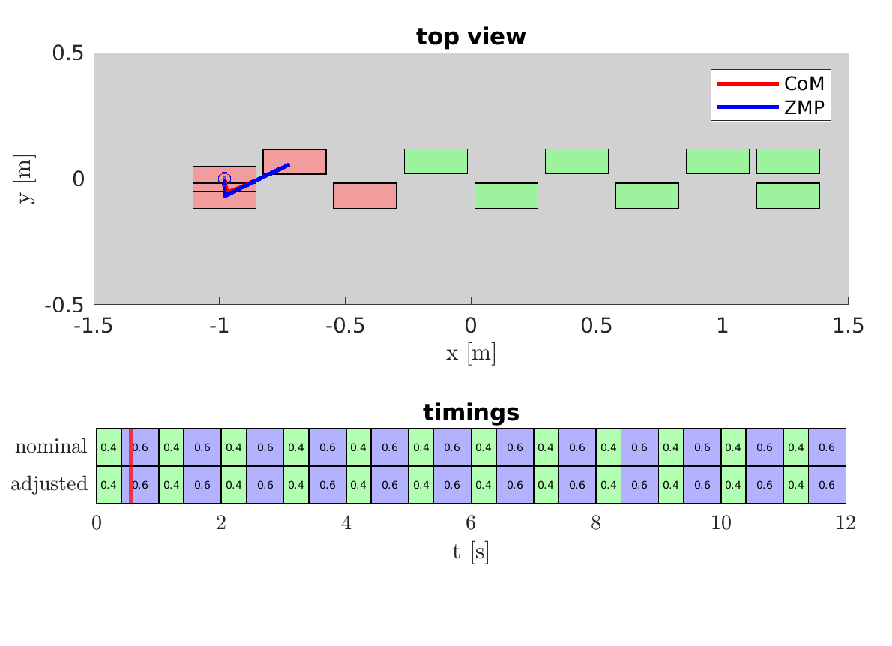
\includegraphics[trim={0 1cm 0 0},clip,width=\textwidth]{figures/empty-fixed-plot-starting.pdf}
    \centering
    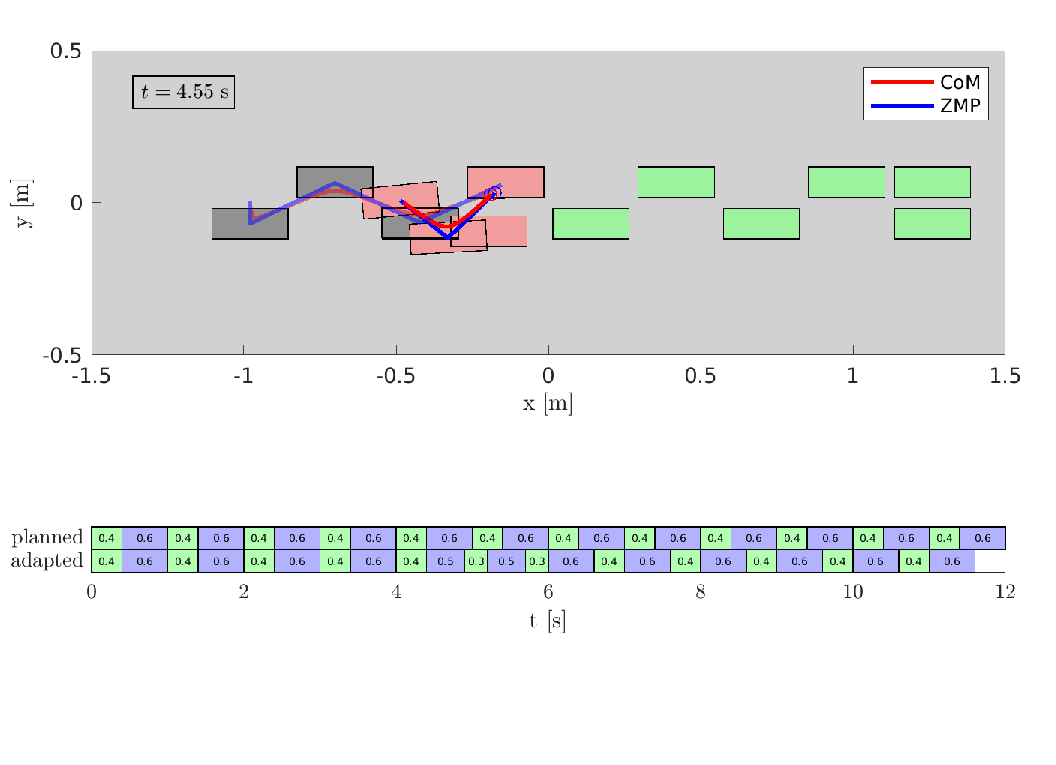
\includegraphics[trim={0 5.9cm 0 0.7cm},clip,width=\textwidth]{figures/empty-fixed-plot-after-push.pdf}
    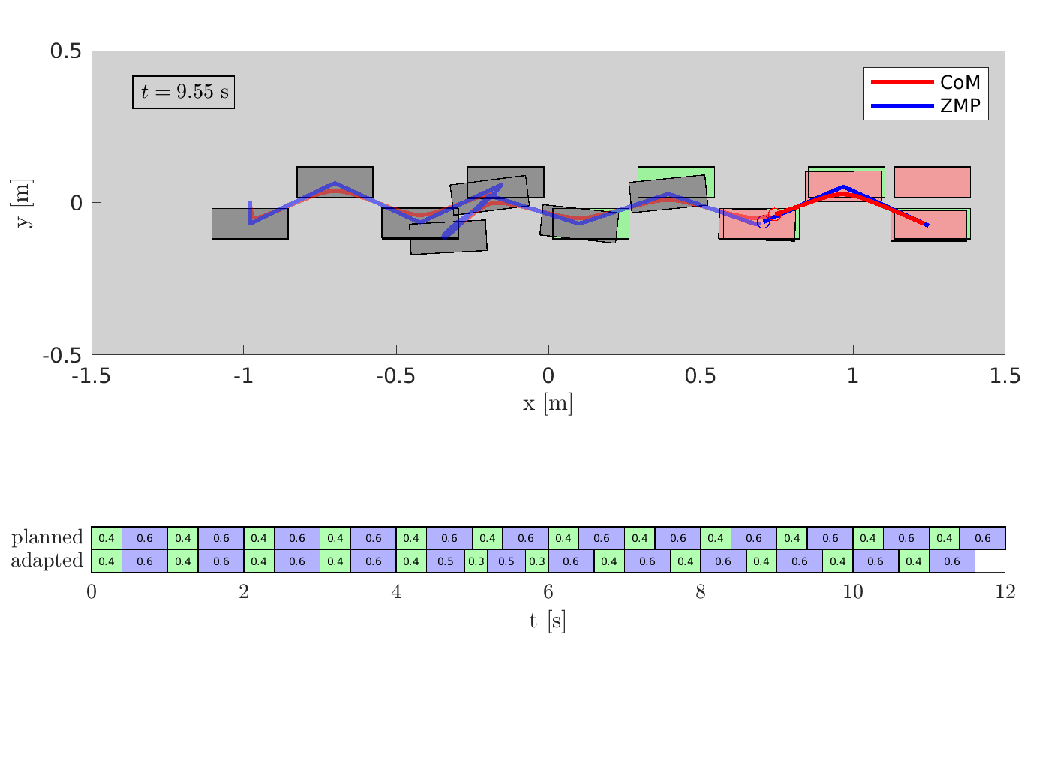
\includegraphics[trim={0 5.9cm 0 0.7cm},clip,width=\textwidth]{figures/empty-fixed-plot-completing-task.pdf}
    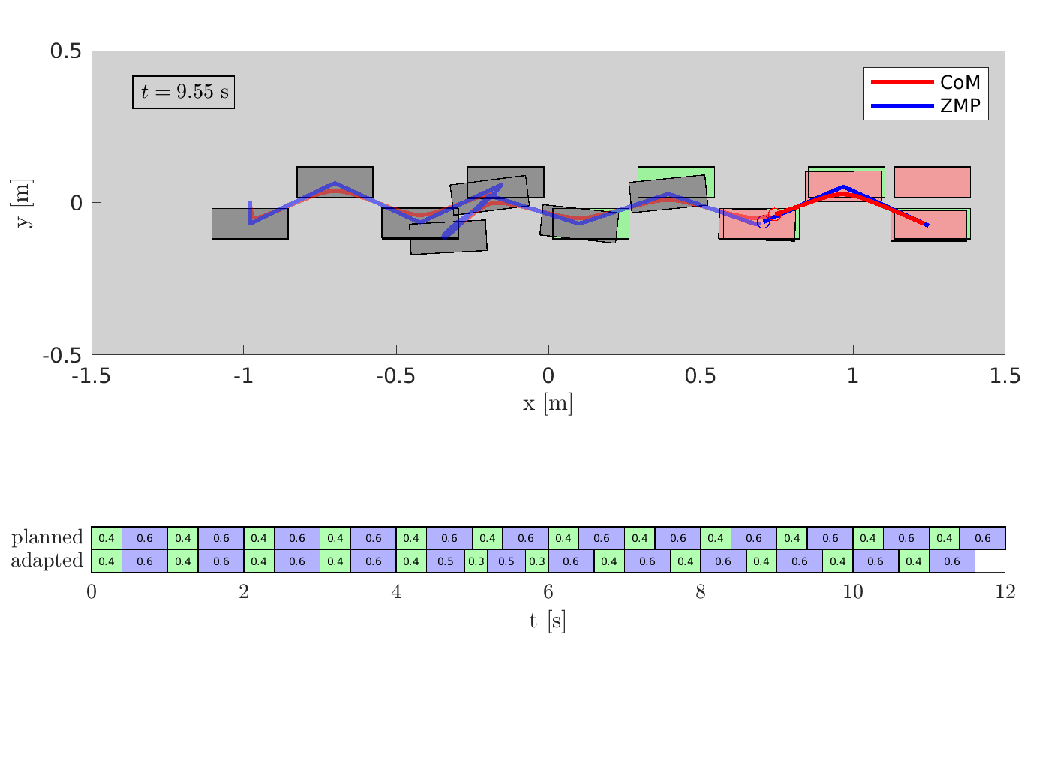
\includegraphics[trim={0 2.2cm 0 8.6cm},clip,width=\textwidth]{figures/empty-fixed-plot-completing-task.pdf}
    \caption{F-FAPA in the {\em empty} scenario. The robot is walking in a
        straight line and is pushed at time $4.5$~[s] (slightly before the first
        snapshot). Green footsteps represent the original candidate plan, while
        the footsteps that are actually executed are shown in grey. Red
        footsteps represent the current adapted subplan. The two bands on the
        bottom show the nominal and adapted timings (green for double support
        and blue for single support). The same color scheme is used for the
        rest of the figures.
    }
    \label{fig:FAPA:matlab_empty}
\end{figure}

\begin{figure}
    \centering
    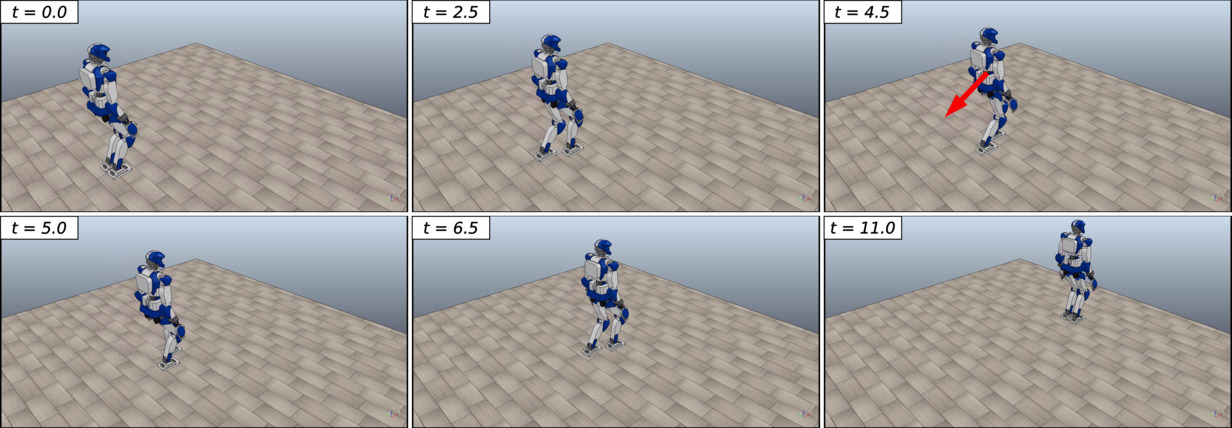
\includegraphics[width=\textwidth]{figures/empty-push-fixed-snapshots.jpeg}
    \caption{HRP-4 walking in the \textit{empty} scenario using F-FAPA.
        The robot walks in a straight line and it is pushed at time 4.5 [s]
        (third snapshot). The robot is able to sustain the push adapting the
        footsteps and the duration of single and double support
        (fourth snapshot), eventually reaching its desired goal (last snapshot).
    }
    \label{fig:FAPA:sim1:snapshots}
\end{figure}

In the second simulation (shown in Fig.~\ref{fig:FAPA:matlab_2pacf}),
the scenario is {\em 2-patches}, and the robot must climb a step.
Upon receiving the push, the footsteps do not change significantly,
because the F-FAPA algorithm is not allowed to move the footstep to the other
patch. As a result, the tolerable push is smaller, i.e., 7.8~[m/s$^2]$.
Figure \ref{fig:FAPA:sim2:snapshots} shows a sequence of snapshots of the
HRP-4 humanoid robot executing the motion.
\begin{figure}
    %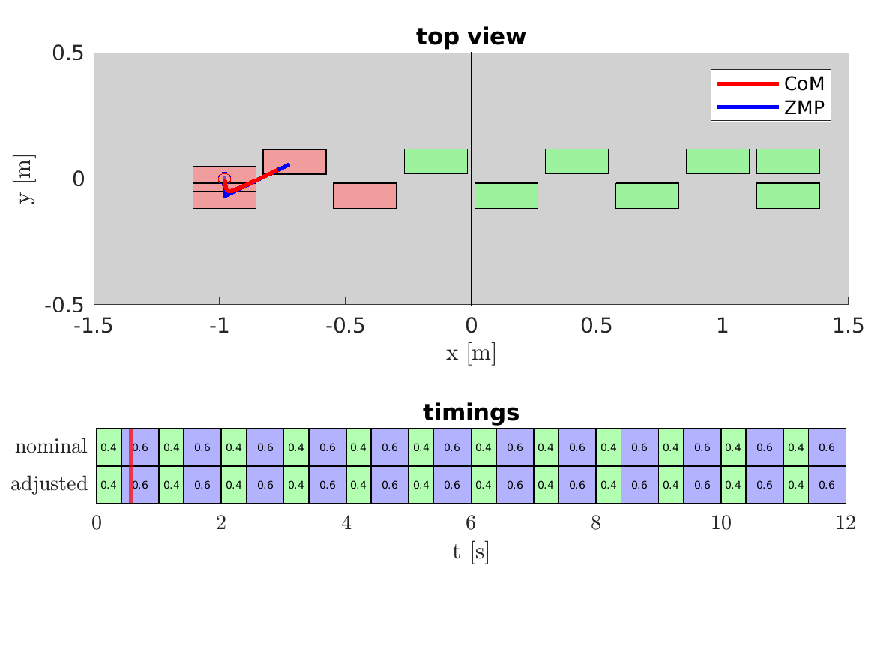
\includegraphics[trim={0 1cm 0 0},clip,width=\textwidth]{figures/two-patches-fixed-plot-starting.pdf}
    \centering
    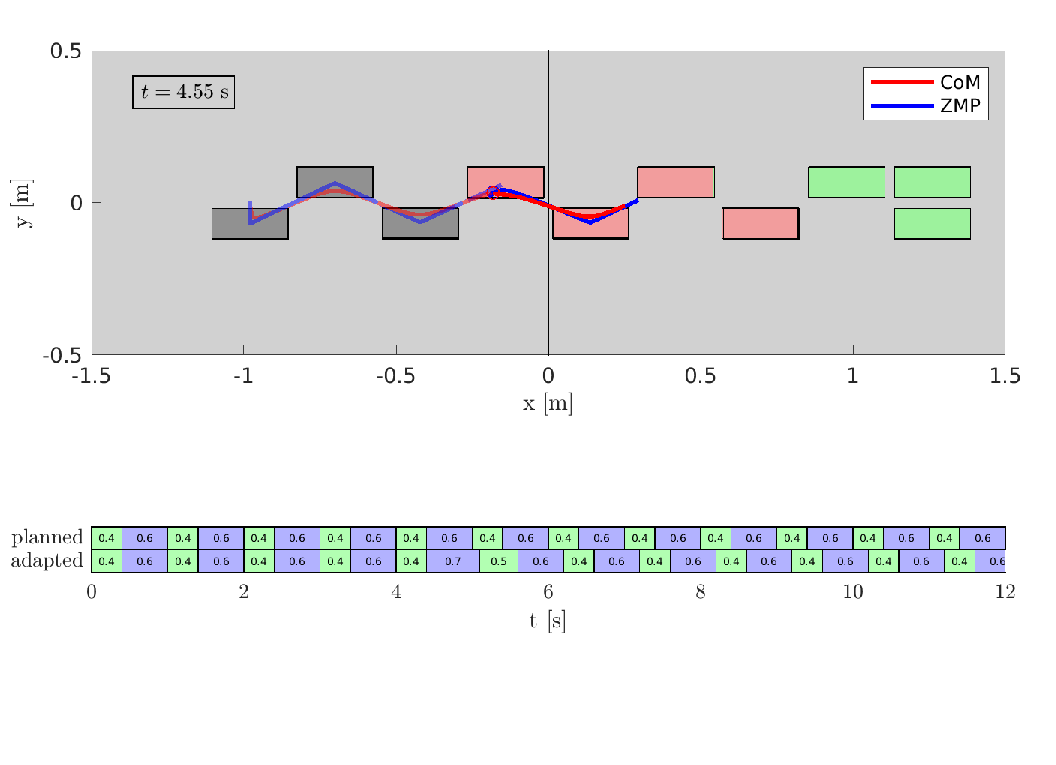
\includegraphics[trim={0 5.9cm 0 0.7cm},clip,width=\textwidth]{figures/two-patches-fixed-plot-after-push.pdf}
    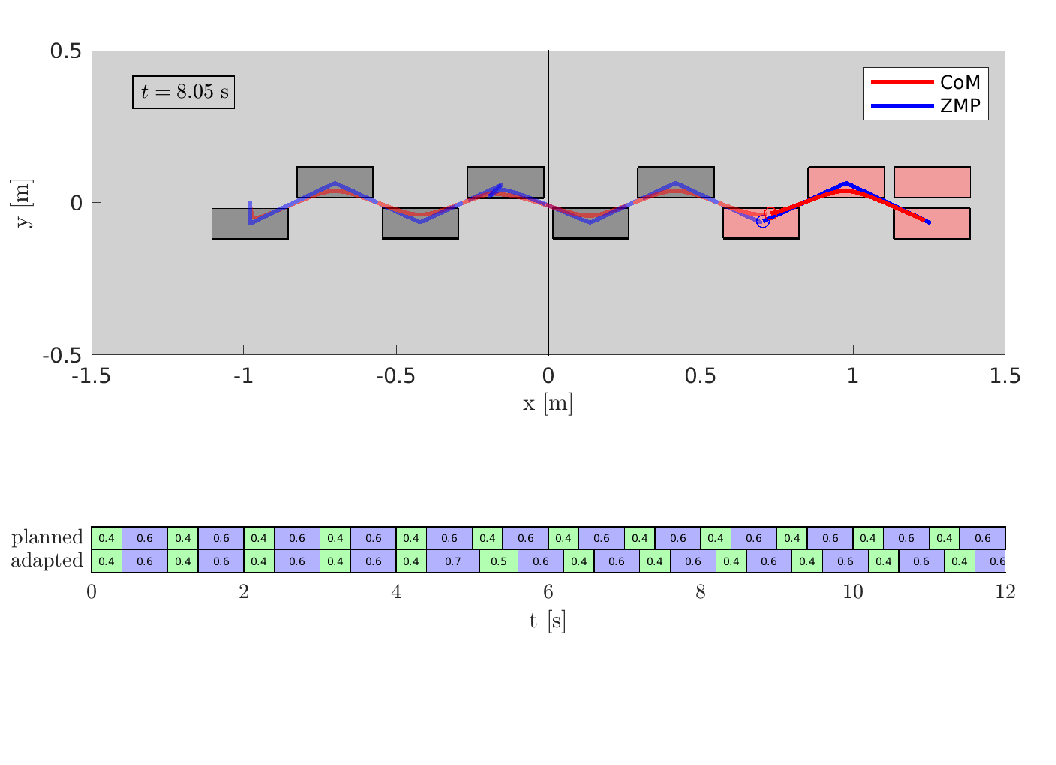
\includegraphics[trim={0 5.9cm 0 0.7cm},clip,width=\textwidth]{figures/two-patches-fixed-completing-task.pdf}
    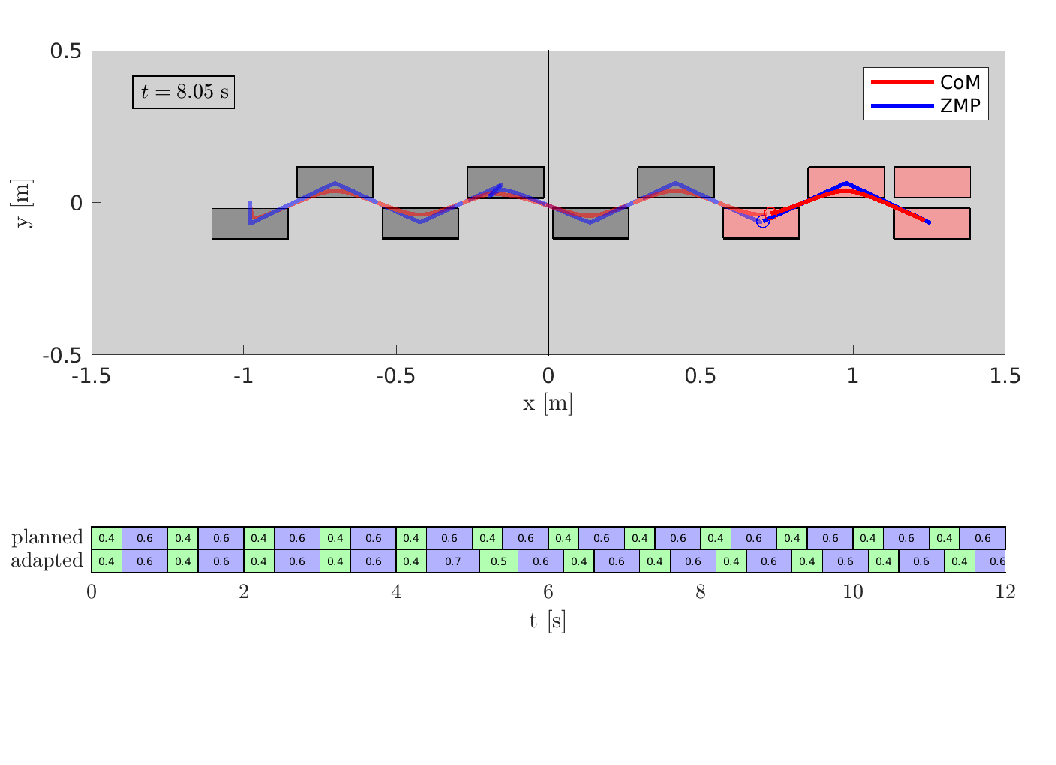
\includegraphics[trim={0 2.2cm 0 8.6cm},clip,width=\textwidth]{figures/two-patches-fixed-completing-task.pdf}
    \caption{F-FAPA in the {\em 2-patches} scenario. The robot is walking in
        a straight line and is pushed at time $4.5$~[s] (slightly before the
        first snapshot). Since changing patches is not allowed, the magnitude
        of the push that can be tolerated is quite small, compared to that of
        the other simulations.
    }
    \label{fig:FAPA:matlab_2pacf}
\end{figure}

\begin{figure}
    \centering
    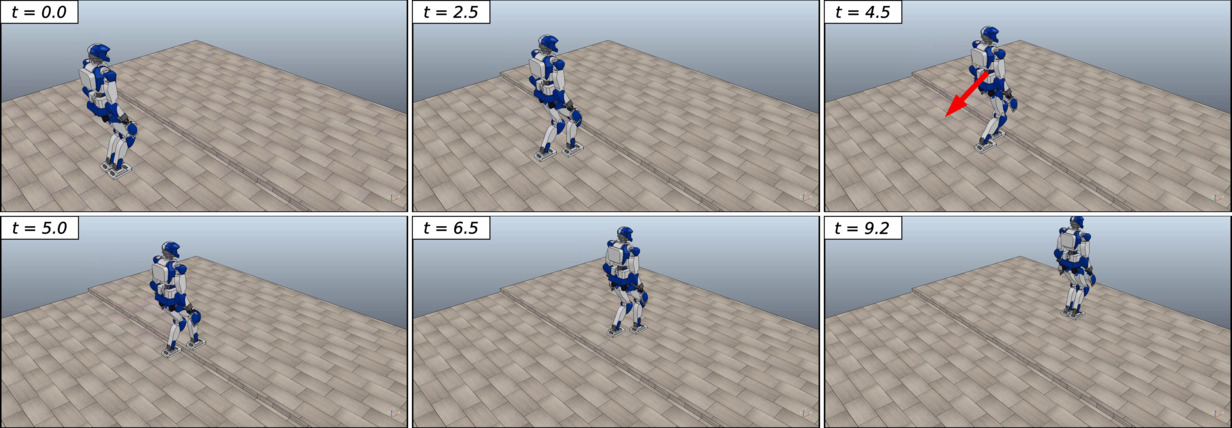
\includegraphics[width=\textwidth]{figures/two-patches-push-fixed-snapshots.jpeg}
    \caption{HRP-4 walking in the \textit{2-patches} scenario using F-FAPA.
        The robot walks in a straight line and it is pushed at time 4.5 [s]
        (third snapshot). The robot is able to sustain the push adapting the
        duration of single and double support (fourth snapshot), eventually
        reaching its desired goal (last snapshot).
    }
    \label{fig:FAPA:sim2:snapshots}
\end{figure}

In the third simulation (shown in Fig.~\ref{fig:FAPA:matlab_2pacmi} ),
the scenario is still {\em 2-patches}, but now the scheme is using V-FAPA.
When the push is perceived, the first predicted footstep is moved to the lower
patch, and as a result the increase of the tolerable push intensity is very
significant, i.e., the same as in the {\em empty} scenario.
Figure \ref{fig:FAPA:sim3:snapshots} shows a sequence of snapshots of
the HRP-4 humanoid robot executing the motion.
\begin{figure}
    %\includegraphics[trim={0 1cm 0 0},clip,width=\textwidth]{figures/two-patches-mixed-integer-plot-starting.pdf}
    \centering
    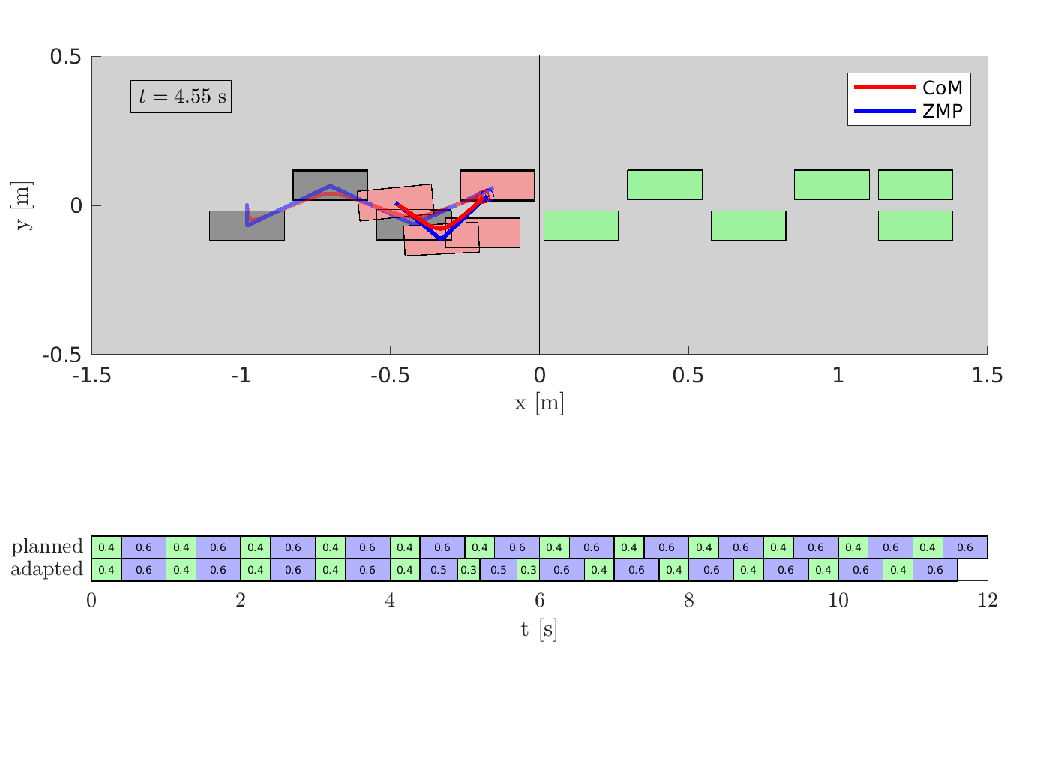
\includegraphics[trim={0 5.9cm 0 0.7cm},clip,width=\textwidth]{figures/two-patches-mixed-integer-after-push.pdf}
    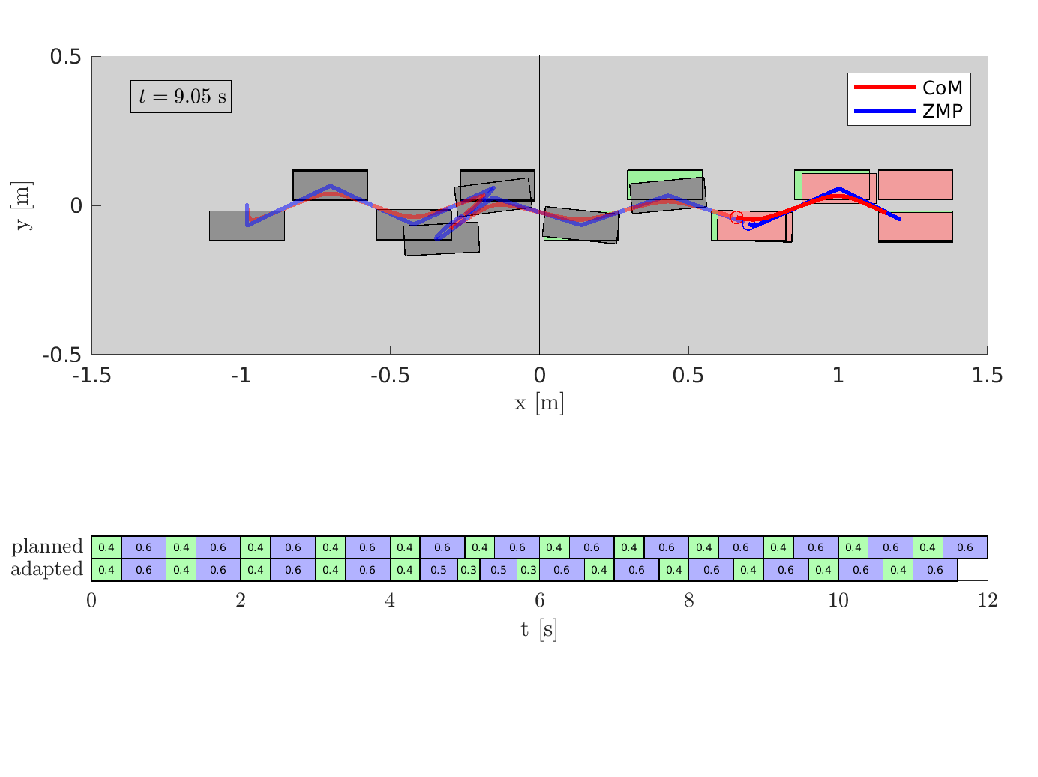
\includegraphics[trim={0 5.9cm 0 0.7cm},clip,width=\textwidth]{figures/two-patches-mixed-integer-completing-task.pdf}
    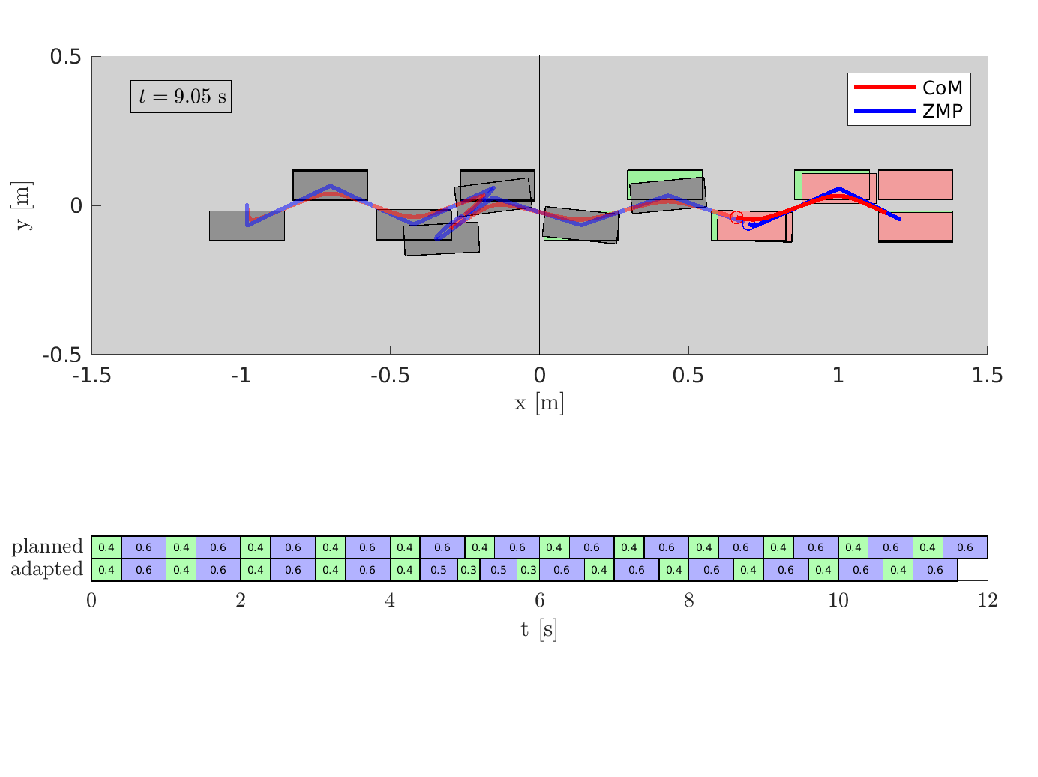
\includegraphics[trim={0 2.2cm 0 8.6cm},clip,width=\textwidth]{figures/two-patches-mixed-integer-completing-task.pdf}
    \caption{V-FAPA in the {\em 2-patches} scenario. The robot is walking
        in a straight line and is pushed at time $4.5$~[s] (slightly before the
        first snapshot). Now the robot is allowed to adapt the footstep position
        to the other patch, and is able to tolerate a stronger push.
    }
    \label{fig:FAPA:matlab_2pacmi}
\end{figure}

\begin{figure}
    \centering
    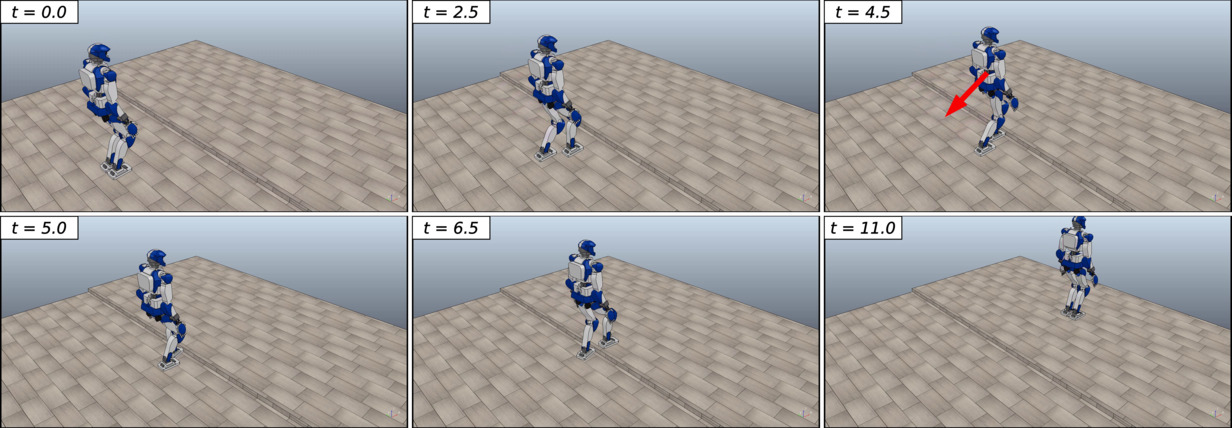
\includegraphics[width=\textwidth]{figures/two-patches-push-mixed-integer-snapshots.jpeg}
    \caption{HRP-4 walking in the \textit{2-patches} scenario using V-FAPA.
        The robot walks in a straight line and it is pushed at time 4.5 [s]
        (third snapshot). The robot is able to sustain the push adapting the
        footsteps and the duration of single and double support (fourth
        snapshot), eventually reaching its desired goal (last snapshot).
        Notice how the robot is able to sustain a stronger push by placing
        the foot in the first patch.
    }
    \label{fig:FAPA:sim3:snapshots}
\end{figure}

In the last simulation, the robot is moving through a more complex environment
constituted by a long staircase. While climbing, the robot is subject to
multiple pushes, triggering several footstep adjustments.
Figure \ref{fig:FAPA:sim1:snapshots} shows a sequence of snapshots of the
HRP-4 humanoid robot executing the motion.
\begin{figure}
    \centering
    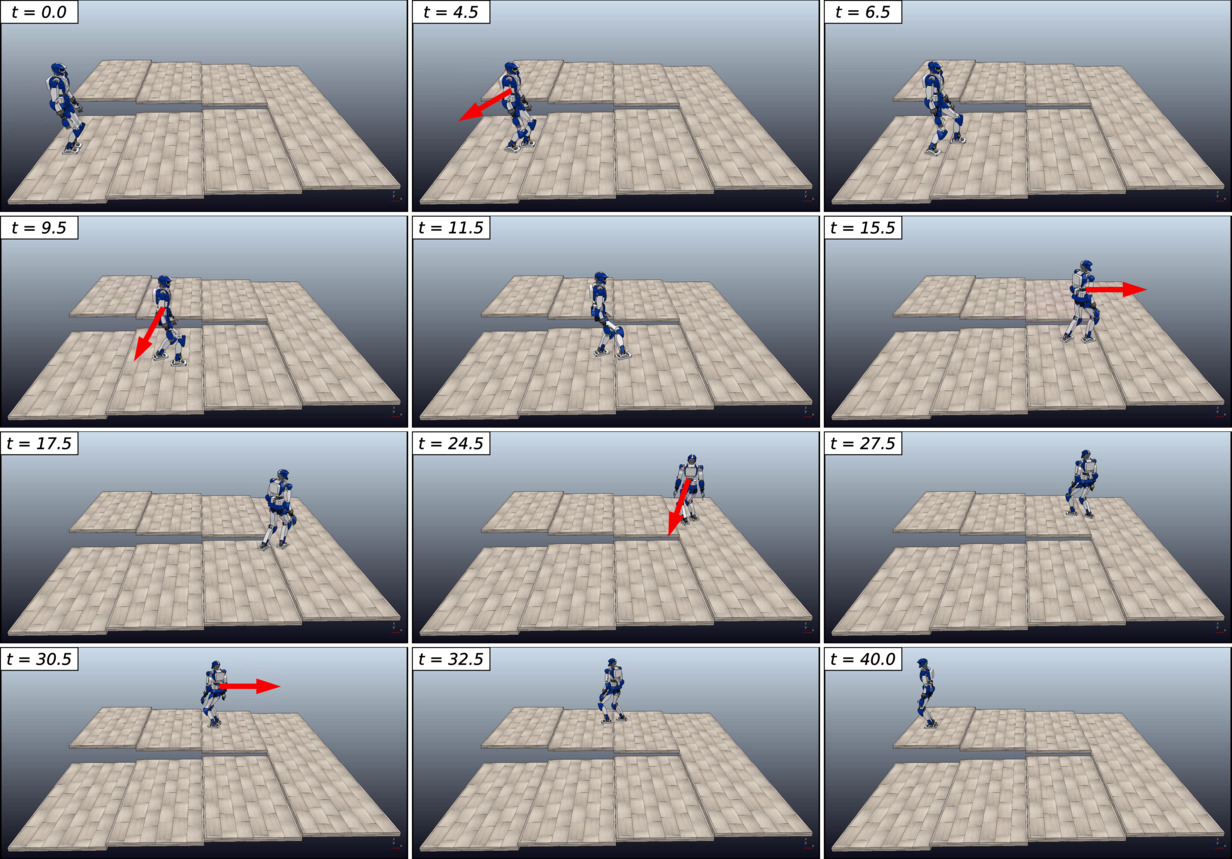
\includegraphics[width=\textwidth]{figures/staircase-multiple-pushes-snapshots.jpeg}
    \caption{HRP-4 walking in a scenario composed of multiple staircases
        using V-FAPA. The robot follows a footstep plan and it is pushed
        multiple times during the execution of the motion (second, fourth,
        sixth , eight and tenth snapshot). The robot is able to sustain
        different pushes adapting the footsteps and the duration of single
        and double support, and changing the patch when necessary.
        Eventually, the robot is able the reach the final patch.
    }
    \label{fig:FAPA:sim3:snapshots}
\end{figure}

\begin{table}
    \centering
    \begin{tabular}{*{6}{c}}
        Algorithm & Solver & Average [s] & Std dev. [s] & Max [s] \\
        \hline
        F-FAPA & IPOPT & 0.0207 & 0.0041 & 0.0467 \\
        F-FAPA & Knitro & 0.0144 & 0.0032 & 0.0329 \\
        V-FAPA & BONMIN & 0.3164 & 0.2075 & 1.2098 \\
        V-FAPA & Knitro & 0.0316 & 0.0393 & 0.3985
    \end{tabular}
    \caption{Performance metrics of F-FAPA in the {\em empty} scenario and
        V-FAPA in the {\em 2-patches} scenario, using different solvers.
    }
    \label{tab:benchmarks}
\end{table}

To discuss the real-time applicability of the scheme, we report performance
metrics in Table~\ref{tab:benchmarks}. The solvers used are IPOPT
and Knitro for F-FAPA, and BONMIN and Knitro for
V-FAPA. Knitro is faster overall, but IPOPT still
demonstrates good performance for F-FAPA, compatible with real-time
requirements. For V-FAPA, BONMIN is clearly too slow, while
Knitro has an average performance that is real-time on average,
but some outliers violate the requirements. Since all results in this chapter
are simulated, real-time performance is desirable but not critical.
However, it is necessary for hardware implementation, which is why we will
be working to guarantee real-time performance in future works.
